\documentclass{article}
\usepackage{tikz}
\usepackage{textcomp,gensymb}
\usepackage{tfrupee}
\usepackage{enumitem}
\graphicspath{{figs/}}

\begin{document}
\begin{center}
    \textbf{ \LaTeX{} Assignment}
\end{center}

\begin{enumerate}
    \item The hour-hand of a clock is 6 cm long.The angle swept by it between 7:20 a.m. and 7:55 a.m. is:

\begin{enumerate}[label=(\alph*)]
    \item $(\frac{35}{4})\degree$
    \item $(\frac{35}{2})\degree$
    \item $35\degree$
    \item $70\degree$
\end{enumerate}

\item In the given figure, $ AB \parallel PQ $.If $AB=6$ cm,$PQ=2$ cm and $OB=3$ cm,then the length of $OP$ is:

\begin{figure}[h]
    \centering
    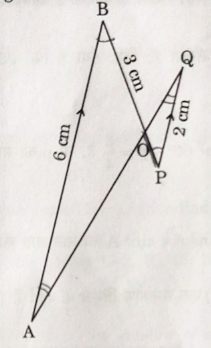
\includegraphics[width=0.3\columnwidth]{figs/30_2_1_Q18.png}
    \caption{}
    \label{fig:30_2_1_Q18}
\end{figure}
\begin{enumerate}[label=(\alph*)]
    \item 9cm
    \item 3cm
    \item 4cm 
    \item 1cm
\end{enumerate}

\item The length of the shadow of a tower on the plane ground is $\sqrt{3}$ times the height of the tower.Find the angle of elevation of the sun.

\item  The angle of elevation of the top of a tower from a point on the ground which is 30 m away from the foot of the tower,is $30\degree$ .Find the height of the tower.

\item  A car has two wipers which do not overlap. Each wiper has a blade of length 21 cm sweeping through an angle of $120\degree$. Find the total area cleaned at each sweep of the two blades.

\item  As observed from the top of a 75 m high lighthouse from the sea-level,the angles of depression of two ships are $30\degree$ and $60\degree$.If one ship is exactly behind the other on the same side of the lighthouse,find the distance between two ships.(Use $\sqrt{3} = 1.73$)

\item  From a point on the ground,the angle of elevation of the bottom and top of a transmission tower fixed at the top of 30 m high building are 30\degree and 60\degree, respectively.Find the height of the transmission tower.(Use $\sqrt{3} = 1.73$)
    
\item Sides $AB$ and $BC$ and median $AD$ of a triangle $ABC$ are respectively proportional to sides $PQ$ and $QR$ and median $PM$ of $\triangle PQR$. Show that $\triangle ABC \sim \triangle PQR$. 

\item  Through the mid-point $M$ of the side $CD$ of a parallelogram $ABCD$,the line $BM$ is drawn intersecting $AC$ in $L$ and $AD$(produced) in $E$.Prove that $EL=2BL$.

\item  In an annual day function of a school,the organizers wanted to give a cash prize along with a memento to their best students. Each memento is made as shown in  the figure and its base $ABCD$ is shown from the front side. The rate of silver plating is \rupee \hspace{4 pt}$20 \hspace{4 pt} per \hspace{ 4 pt}  cm^2$.

\begin{figure}[h]
    \centering
    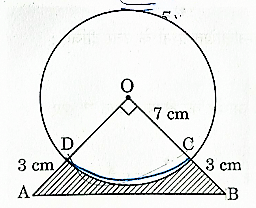
\includegraphics[width=0.5\columnwidth]{figs/30_2_1_Q36.png}
    \caption{memento}
    \label{fig:img2}
\end{figure}

Based on the above, answer the following questions:
\begin{enumerate}[label=(\roman*)]
    \item What is the area of the quadrant $ODCO$?
    \item Find the area of $\triangle  AOB$.
    \item What is the total cost of silver plating the shaded part $ABCD$?
    \item what is the length of arc $CD$?
\end{enumerate}


\end{enumerate}
\end{document}
